
\documentclass[12pt]{article}
\usepackage{amsmath}
\usepackage{amsfonts}
\usepackage{mathrsfs}
\usepackage{lscape}
\usepackage{listings}
\usepackage{graphicx} % Allows for importing of figures
\usepackage{color} % Allows for fonts to be colored
\usepackage{comment} % Allows for comments to be made
\usepackage{accents} % Allows for accents to be made above and below text
%\usepackage{undertilde} % Allows for under tildes to take place for vectors and tensors
\usepackage[table]{xcolor}
\usepackage{array,ragged2e}
\usepackage{hyperref}
\usepackage{framed} % Allows boxes to encase equations and such
\usepackage{subcaption} % Allows for figures to be side-by-side
\usepackage{float} % Allows for images to not float in the document
\usepackage{booktabs}
%\usepackage[margin=0.75in]{geometry}
\usepackage[final]{pdfpages}
\usepackage{enumitem}
\usepackage[section]{placeins}

%%%%%%%%%%%%%%%%%%%%%%%%%  Function used to generate vectors and tensors %%%%%%%%%
\usepackage{stackengine}
\stackMath
\newcommand\tensor[2][1]{%
	\def\useanchorwidth{T}%
	\ifnum#1>1%
	\stackunder[0pt]{\tensor[\numexpr#1-1\relax]{#2}}{\scriptscriptstyle \sim}%
	\else%
	\stackunder[1pt]{#2}{\scriptscriptstyle \sim}%
	\fi%
}
%%%%%%%%%%%%%%%%%%%

\definecolor{mygrey}{rgb}{0.97,0.98,0.99}
\definecolor{codeblue}{rgb}{.2,0,1}
\definecolor{codered}{rgb}{1,0,0}
\definecolor{codegreen}{rgb}{0.3,0.33,0.12}
\definecolor{codegray}{rgb}{0.5,0.5,0.5}
\definecolor{codepurple}{rgb}{0.55,0.0,0.55}
\definecolor{codecyan}{rgb}{0.0,.4,.4}

\lstdefinestyle{mystyle}{
	backgroundcolor=\color{mygrey},   
	commentstyle=\color{codegreen},
	keywordstyle=\color{codeblue},
	stringstyle=\color{codepurple},
	numberstyle=\tiny\color{codegray},
	basicstyle=\footnotesize,
	breakatwhitespace=false,         
	breaklines=true,                 
	captionpos=b,                    
	keepspaces=true, 
	numbers=left,                    
	numbersep=5pt,                  
	showspaces=false,                
	showstringspaces=false,
	showtabs=false,                  
	tabsize=2
}
\lstset{style=mystyle}

\lstset{language=Matlab,backgroundcolor=\color{mygrey}}
\usepackage{lastpage}
\usepackage{fancyhdr}
\pagestyle{fancy}
%\lhead{\large{Nik Benko, John Callaway, Nick Dorsett, Martin Raming}} 
%\chead{\large{\textbf{ME EN 6960: Lab 1}}}
%\rhead{\today}
\cfoot{[\thepage\ of \pageref{LastPage}]}
\fancyheadoffset{.5cm}
\setlength{\parindent}{0cm}
\usepackage[left=.5in, right=0.50in, top=1.00in,bottom=1.00in]{geometry}
\usepackage{microtype} 
\usepackage{setspace}
\doublespace
%%%%%%%%%%%%%%%%%%%%%%%%%%%%%%%%%%%%%%%%%%%%%%%%%%%%%%%%%%%%%%%%%%%%%%%%%%
% git testing ii

\begin{document}
\title{ Determination of Dynamic Tensile Strength of Concrete Brazil Disc Specimens Using a Split Hopkinson Pressure Bar  \\ \normalsize{ME EN 6960}}
\author{Nik Benko, John Callaway, Nick Dorsett, Martin Raming}
\maketitle

% Nik
\begin{abstract} 

\end{abstract}

\section{Introduction} % Nik

\section{Methods}

\subsection{Experimental Techniques} 

\subsubsection {Split Hopkinson Pressure Bar} % Nick
%Gas gun, bar, location, etc
\subsubsection{High Strain Rate Data Acquisition} % Nick
%Strain gauges, scope

\subsubsection{Statistical Analysis} % John

Central tendency and dispersion are two common ways to quantify the distribution of a data set (ref). Central tendency is quantified using the measures of mean and median. The mean of a data set is given by
\begin{equation}
\bar{x} = \sum_{i=1}^{n}\frac{x_{i}}{n}
\end{equation}
where $\bar{x}$ is the mean, $n$ is the number of data points and $x_{i}$ is the ith data point. The median is the central value of an ordered set of the data. Dispersion represents the distribution of data around the central tendency, usually the mean. Dispersion is measured using standard deviation and variance, given by 
\begin{equation}
S_{x} = \left[\sum_{i=1}^{n}\frac{\left(x_{i}-\bar{x}\right)^2}{n-1}\right]^\frac{1}{2}
\end{equation}  
\begin{equation}
S_{x}^2 = \sum_{i=1}^{n}\frac{\left(x_{i}-\bar{x}\right)^2}{n-1}
\end{equation} 
where $S_{x}$ is the standard deviation and $S_{x}^2$ is the variance.

For experiments involving strength of materials due to brittle fracture, a Weibull distribution function can be applied to show the probability of failure at a given strength value (ref). The Weibull Distribution is given by
\begin{equation}
p(x) = 1-e^{-\left[\frac{\left(x-x_{o}\right)}{b}\right]^m} \text{ for } x > x_{o}
\end{equation}
\begin{equation}
p(x) = 0  \text { for } x < x_{o}
\end{equation} 
where $p(x)$ is the probability of failure occurring at $x$, $x_{o}$ is the zero strength value of the distribution, $b$ is scale parameter and $m$ is the Weibull slope parameter. The values of distribution parameters $x_{o}$, $b$ and $m$ can be determined iteratively or by use of a commercial software such as MATLAB. MATLAB has a built in function, $wblfit$. that generates the Weibull parameters and probability distribution function with a 95\% confidence interval (ref).

\subsection{Procedure} % John

Concrete Brazil Disc specimens with a diameter of xx mm and thickness of xx mm were loaded in a SHPB test setup. The SHPB utilized 19.05 mm diameter aluminum 7075-T6 bars for the incident and transmitted bars. The incident bar length was 2.438 m and the transmitted bar length was 1.930 m. Aluminum platens with a matching acoustic impedance were attached to the loading end of the incident and transmitted bars to prevent damage to the SHPB apparatus from the concrete specimens. A 1.058 mm thick, 9.525 mm diameter lead pulse shaper was placed on the non-loading end of the incident bar for each test. The striker bar was propelled using a REL gas gun. The experimental setup can be seen in Figure \ref{fig:TestSetup}.
\\ \\
Initial calibration and bar wave speed were determined without specimens using a gas gun pressure of 10.2 psi. A total of ten specimens were tested at four separate gas gun pressures - 8, 9, 10.2 and 12.4 psi. Strain gauges attached to both the incident and transmitted bars were used to detect the incident, reflected and transmitted waves in the bar. The strain gauges were located 1.219 m from the loading point on the incident bar and 0.965 m from the loading point on the transmitted bar. Voltage outputs from the strain gauges were collected using a Tektronix DPO 2004B oscilloscope. All analysis was completed in MATLAB.   

\subsection{Error and Uncertainties} % Nick 

\section{Results} % Martin

\section{Discussion} % Martin

\section{Conclusion} % Nik

% Bar speed and strain rate % Martin
% Forward and backward propogation of waves % Nick
% Conversion of voltage to strain, strain to force, force to strength % Nick
% Statistical Analysis % John

\section{Figures}
\begin{figure}[H]
	\centering
	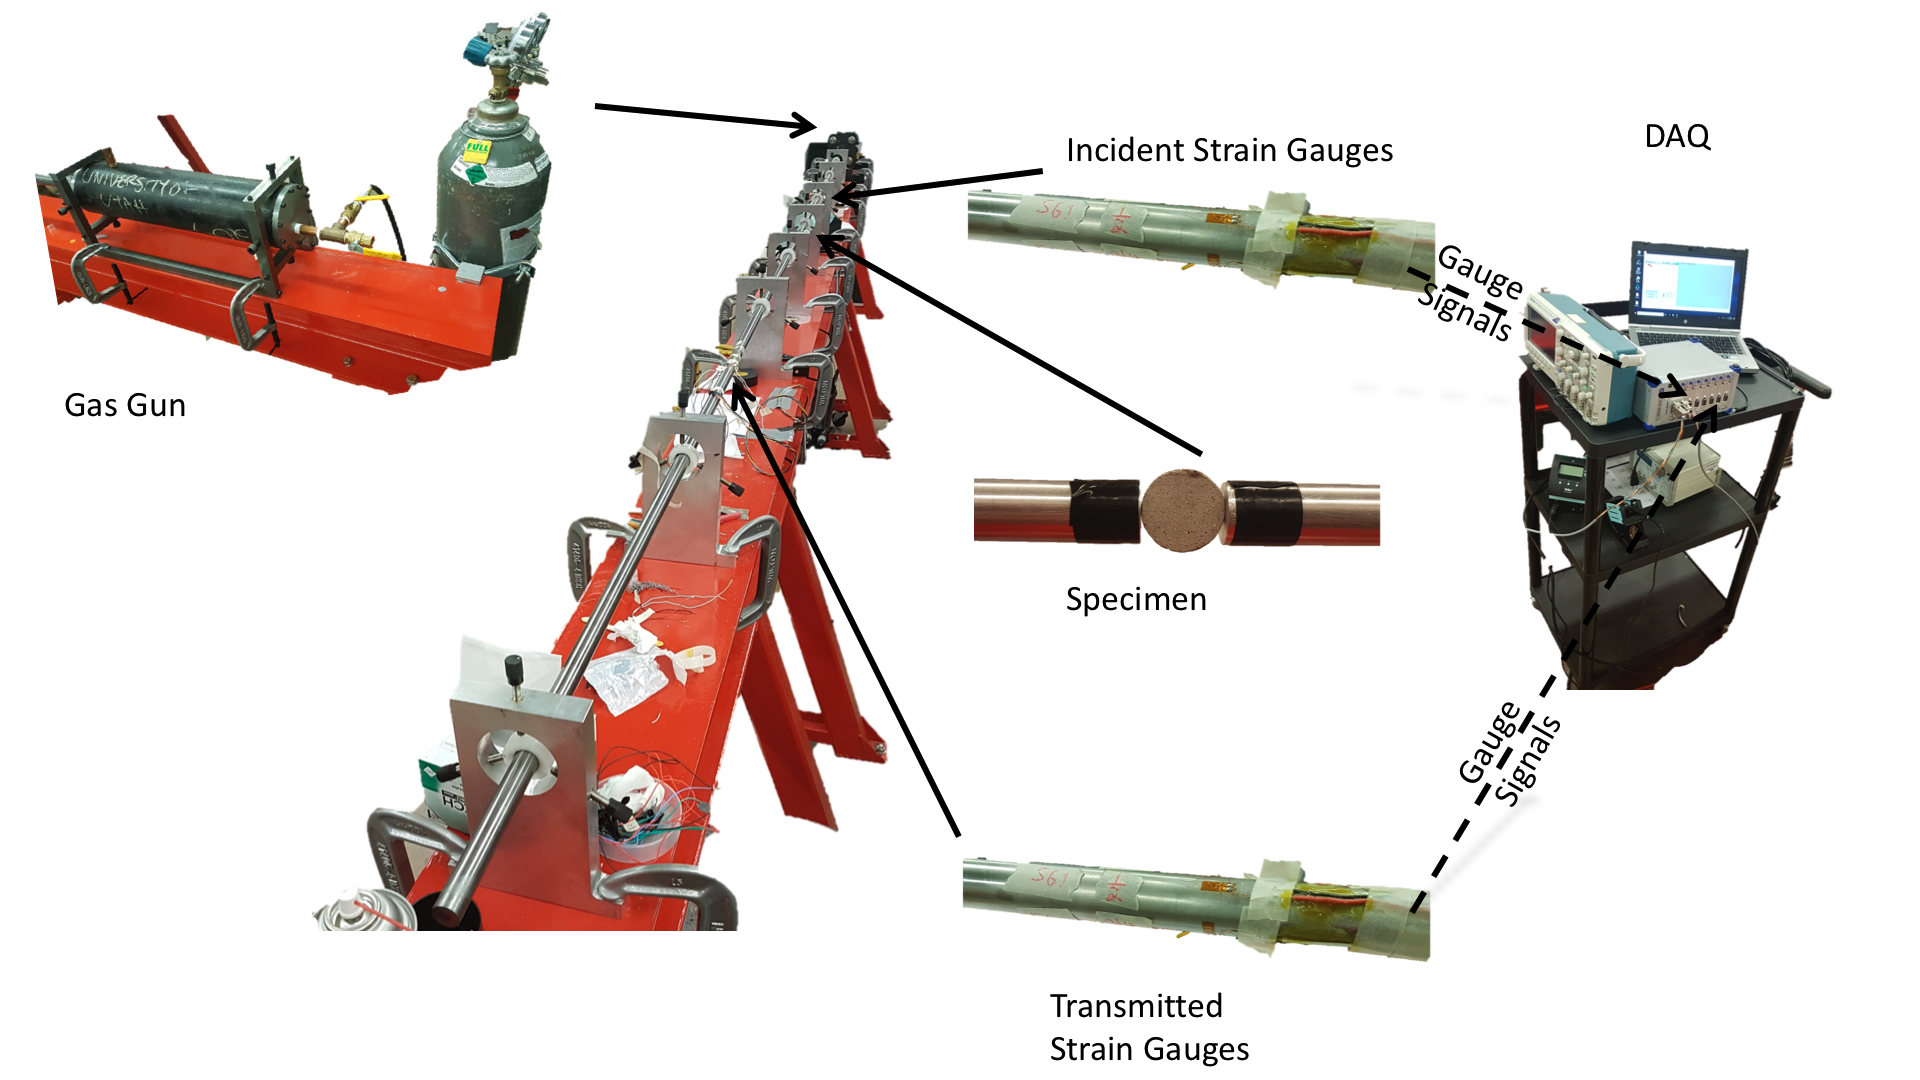
\includegraphics[width=1\textwidth]{TestSetUp.png}
	\caption{Experimental setup of the Split Hopkinson Pressure Bar}
	\label{fig:TestSetup}
\end{figure}


\section{Tables}
%Recoded Experimental Data:
%\begin{table}[h]\footnotesize
%	\centering
%	\begin{tabular}{ |l|l|l|l| }
%		\hline
%		\multicolumn{2}{|c|}{\textbf{Mode I}}&\multicolumn{2}{|c|}{\textbf{Mixed Mode}}\\ \hline
%		\textbf{Load [N]} & \textbf{Image Number}&\textbf{Load [N]} & \textbf{Image Number}\\  \hline
%		0-5 & 7.784 & 0-4 & 25.58 \\ \hline
%		6& 7.784 & 5 & 27.58 \\ \hline
%		7 & 93.77 & 6 & 86 \\ \hline
%		8 & 215.6 & 7 &191.7 \\ \hline
%		9 & 295 & 8 & 324 \\ \hline
%		10 & 412 & 9 & 431 \\ \hline
%		11 & 489.6 & 10 & 486 \\ \hline
%		12 & 587 & 11 & 534.7 \\ \hline
%		13 & 745 & 12 & 629.1 \\ \hline
%		14 & 834 & 13 & 761.7 \\ \hline
%		15 & 899 & 14 & 805.3 \\ \hline
%		16 & 952 & 15 & 849.6 \\ \hline
%		17 & 1010 & 16 & 896 \\ \hline
%		-	& - & 17 & 1000 \\ \hline
%		
%		
%		
%	\end{tabular}
%	\caption{Loads and associated image number, first few images were used as reference images.}
%	\label{tab:data}
%\end{table}
%% All layups
%\
%\section{Appendix}
%
%%\subsection{Code}
%%
%%\begin{verbatim}
%%
%%\end{verbatim}
%
%\newpage
\bibliographystyle{IEEEtran}
\bibliography{Lab2Bib}
\end{document}